\documentclass[tikz,border=10pt]{standalone}
\usepackage{pgfplots}
\pgfplotsset{compat=1.18}

\begin{document}
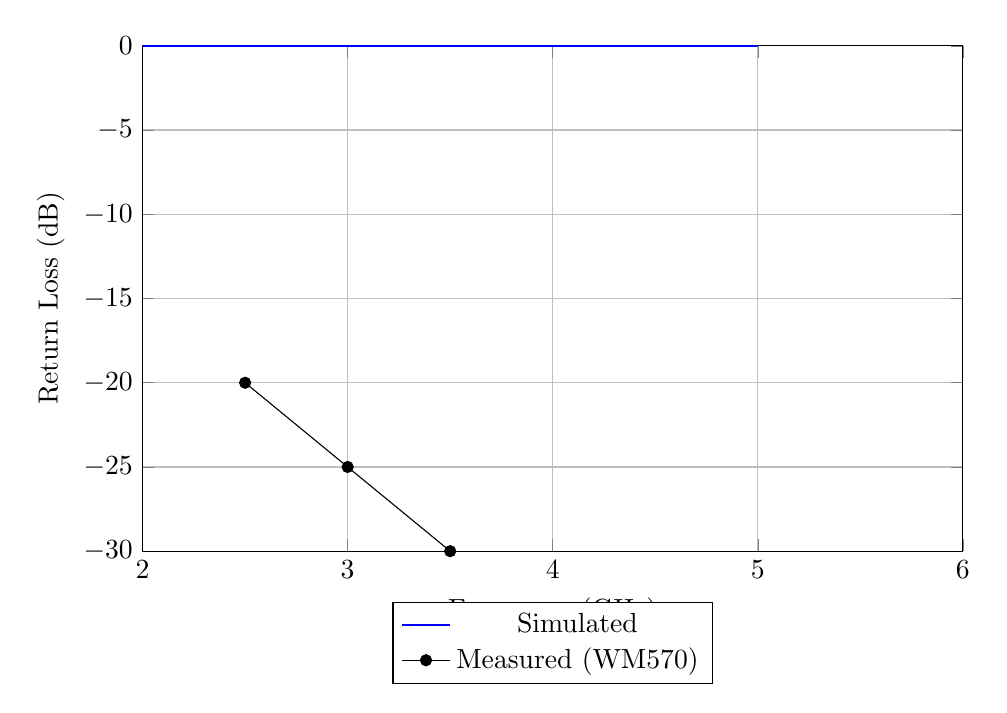
\begin{tikzpicture}
    \begin{axis}[
        width=12cm,
        height=8cm,
        xlabel={Frequency (GHz)},
        ylabel={Return Loss (dB)},
        grid=major,
        legend style={at={(0.5,-0.1)}, anchor=north},
        ytick distance=5,
        xtick distance=1,
        ymin=-30,
        ymax=0,
        xmin=2,
        xmax=6,
        samples=100,
        ]
        
        % Simulated data
        \addplot[blue, thick] {-(1/(4*pi*sqrt(1e9*x^2)))}; 
        \addlegendentry{Simulated};
        
        % Measured data (example points)
        \addplot[black, mark=*] coordinates {(2.5, -20) (3, -25) (3.5, -30) (4, -35) (4.5, -40)};
        \addlegendentry{Measured (WM570)};
    \end{axis}
\end{tikzpicture}
\end{document}